\chapter{\sc Two-Phase Navier--Stokes Flow Numerical Results}
\label{ch:ns_results}
In order to test our method, and to allow comparisons with the unfitted finite
element approximation in \cite{fluidfbp}, we now present several numerical
experiments in 2d and 3d.

\section{Exact solutions}\label{sec:ns_exact_solutions}
Let $\Gamma(t) = \{ \vec z \in \R^d : |\vec z\,| = r(t)\}$ be a sphere of radius
$r(t)$ and curvature $\varkappa(t) = -\,\frac{d-1}{r(t)}$. Moreover let
$\alpha,\alpha_1,\alpha_2,\gamma\in \R_{\geq 0}$ be given. Here, we also allow
non divergence-free problem. Therefore, for the non divergence-free cases, the
incompressibility condition (\ref{eq:ns_full_mass}) is replaced by
\begin{equation}\label{eq:ns_compressible}
\nabla\,.\,\vec u = f_{\rm{div}}\,.
\end{equation}

\subsection{Expanding bubble I}
The expanding sphere where
\begin{subequations}
\begin{equation} \label{eq:ns_sol_1_r}
r(t) = \mathrm{e}^{\alpha\,t}\,r(0)\,,
\end{equation}
together with
\begin{equation} \label{eq:ns_sol_1_up}
\vec u(\vec z, t) = \alpha\,\vec z \,, \quad
p(\vec z, t) = -\,\bigg(\gamma - 2\,\alpha\,\frac{\mu_+ - \mu_-}
{d-1}r(t)\bigg)\,\varkappa(t)\,\left[ \charfcn{\Omega_-(t)} -
\frac{\vol(\Omega_-(t))}{\vol(\Omega)}\right],
\end{equation}
\end{subequations}
is an exact solution to the problem (\ref{eq:ns_full_momentum}--i), with
(\ref{eq:ns_full_mass}) replaced by (\ref{eq:ns_compressible}), on
e.g.\ $\Omega = (-1,1)^d$  with $\vec f(\vec z, t) = \rho\,\alpha^2\,\vec z$,
$f_{\rm{div}} = \alpha\,d$ and $\vec g = \alpha\,\vec z$ on
$\partial_1\Omega=\partial\Omega$.

We now verify that (\ref{eq:ns_sol_1_r},b) is indeed an exact solution. Firstly,
given that
\begin{equation*}
\frac{\partial u_i}{\partial z_j}=\alpha\delta_{ij}\,,
\end{equation*}
the components of the rate-of-deformation tensor are simply
\begin{equation*}
\big[\mat D(\vec u) \big]_{ij} = \frac{1}{2}\bigg(\frac{\partial
u_i}{\partial z_j} + \frac{\partial u_j}{\partial
z_i}\bigg)=\alpha\delta_{ij}\,,
\end{equation*}
and it holds
\begin{align*}
\nabla\,.\,\mat D(\vec u) = \vec 0\,,
\end{align*}
Therefore, given that the pressure $p$ is constant in each phase and that
$\vec u$ does not depend on time, the momentum equation
(\ref{eq:ns_full_momentum}) reduces simply to
\begin{align*}
\rho(\vec u \,.\, \nabla)\vec u=\rho\,\alpha^2\,\vec z
\end{align*}
which is indeed the value of forcing term $\vec f$. Also the non
divergence-free continuity equation (\ref{eq:ns_compressible}) is satisfied
since we have
\begin{equation*}
\nabla\,.\,\vec u=\sum_{j=1}^d\frac{\partial u_j}{\partial z_j} =
\sum_{j=1}^d\alpha=\alpha d \,,
\end{equation*}
which is indeed equal to $f_{\rm{div}}$.
Moreover, also the stress balance
(\ref{eq:ns_full_jump_stress}) holds since, substituting
(\ref{eq:ns_sol_1_up}) in (\ref{eq:ns_full_jump_stress}), we obtain for the
$i$ component
\begin{align*}
& [[2\mu \mat D(\vec u)\,.\,\vec\nu - p\,\vec \nu]_i]_-^+ =
\bigg[2\mu \sum_{j=1}^d\frac{\partial u_i}{\partial z_j}\nu_j - p\nu_i\bigg]_-^+
= \bigg[2\mu\sum_{j=1}^d\alpha\delta_{ij}\nu_j\bigg]_-^+
-\bigg[p\nu_i\bigg]_-^+ \\
& \qquad = \bigg[2\mu\alpha\nu_i\bigg]_-^+
-\bigg(\gamma -2 \alpha \frac{\mu_+ - \mu_-}{d-1}r\bigg)\varkappa\nu_i \\
& \qquad = 2\alpha(\mu_+-\mu_-)\nu_i -\gamma \varkappa \nu_i +
2\alpha\frac{\mu_+ - \mu_-}{d-1}r\frac{1-d}{r}\nu_i \\
& \qquad = 2\alpha(\mu_+-\mu_-)\nu_i -\gamma \varkappa \nu_i -
2\alpha(\mu_+-\mu_-)\nu_i = -\gamma \varkappa \nu_i\,.
\end{align*}
Finally, the dynamic interface condition (\ref{eq:ns_full_velocity}) is
satisfied since the fluid velocity on the interface along the normal direction
is
\begin{equation*}
\vec u\,.\,\vec \nu \!\mid_\Gamma=\alpha\vec z\,.\, \frac{\vec z}{|\vec z\,|} =
\alpha|\vec z\,|=\alpha r\,,
\end{equation*}
while the interface velocity along the normal direction is
\begin{equation*}
\V\,.\,\vec \nu=r^\prime=\alpha r\,.
\end{equation*}

\subsection{Expanding bubble II}
The expanding sphere where
\begin{subequations}
\begin{equation} \label{eq:ns_sol_2_r}
r(t) = \mathrm{e}^{\alpha_1\,t}\,r(0)\,,
\end{equation}
together with
\begin{align} \label{eq:ns_sol_2_up}
& \vec u(\vec z, t) = \bigg(\alpha_1+\alpha_2\charfcn{\Omega_+(t)}(|\vec
z|^2-r(t)^2)\bigg)\,\vec z\,, \\
& p(\vec z, t) = -\,\bigg(\gamma - 4\,\alpha_2\,\frac{\mu_+}{d-1}r(t)^3
\bigg)\,\varkappa(t)\,\left[ \charfcn{\Omega_-(t)} -
\frac{\vol(\Omega_-(t))}{\vol(\Omega)}\right],
\end{align}
\end{subequations}
is an exact solution to the problem (\ref{eq:ns_full_momentum}--i), with
(\ref{eq:ns_full_mass}) replaced by (\ref{eq:ns_compressible}), on e.g.\ $\Omega
= (-1,1)^d$ with
\begin{align}
\vec f(\vec z, t) = &
\rho\,\bigg(\alpha_1^2\,+\charfcn{\Omega_+(t)}\bigg(-2\alpha_1\alpha_2r(t)^2 +
2\alpha_1\alpha_2\big(2|\vec z\,|^2-r(t)^2\big) \nonumber \\
& +\alpha_2^2\big(|\vec z\,|^2-r(t)^2\big)\big(3|\vec z\,|^2 -
r(t)^2\big)-4(d+1)\alpha_2\frac{\mu_+}{\rho}\bigg)\bigg)\vec z\,, \\
f_{\rm{div}} = & \big( \alpha_1
+ \alpha_2\charfcn{\Omega_+(t)}\big(\frac{2+d}{d}|\vec z\,|^2-r(t)^2\big)\big)d
\end{align}
and
\begin{equation}
\vec g = \bigg(\alpha_1+\alpha_2\charfcn{\Omega_+(t)}(|\vec
z|^2-r(t)^2)\bigg)\,\vec z
\end{equation}
on $\partial_1\Omega=\partial\Omega$.

\subsection{Expanding bubble III}
A nontrivial divergence free and radially symmetric solution $\vec u$
can be constructed on a domain that does not contain the origin. To this end,
consider e.g.\ $\Omega = (-1,1)^d \setminus [-\frac13, \frac13]^d$. Then, the
expanding sphere where
\begin{subequations}
\begin{equation} \label{eq:ns_sol_3_r}
r(t) = ([r(0)]^d + \alpha\,t\,d)^\frac1d \,,
\end{equation}
together with
\begin{equation} \label{eq:ns_sol_3_up}
\vec u(\vec z, t) = \alpha\,\frac{\vec z}{|\vec z\,|^d}\,, \quad
p(\vec z, t) = -\,\bigg(\gamma +2\,\alpha\,\frac{\mu_+ - \mu_-}
{r(t)^{d-1}}\bigg)\,\varkappa(t)\,\left[ \charfcn{\Omega_-(t)} -
\frac{\vol(\Omega_-(t))}{\vol(\Omega)}\right],
\end{equation}
\end{subequations}
is an exact solution to the problem (\ref{eq:ns_full_momentum}--i) with
$\vec f(\vec z, t) = \rho\,(1-d)\alpha^2\frac{\vec z}{|\vec z\,|^{2d}}$ and
$\vec g(\vec z) = \alpha\,|\vec z\,|^{-d}\,\vec z$ on
$\partial_1\Omega=\partial\Omega$.

We notice that the exact solution (\ref{eq:ns_sol_3_r},b) is identical to the
expanding bubble solution of the two-phase Stokes problem presented in
\S\ref{sec:stokes_expanding}. The only change is the forcing term $\vec f$
which is now inhomogeneous. Therefore, in order to verify that
(\ref{eq:ns_sol_3_r},b) is indeed an exact solution also to the two-phase
Navier--Stokes problem, it is sufficient to check that the time derivative plus
the convective term in the momentum equation (\ref{eq:ns_full_momentum}) add up
to $\vec f$. Firstly, we compute the $i$ component of the convective term as
\begin{align*}
\big[(\vec u \,.\, \nabla)\vec u\big]_i =&
\sum_{j=1}^d\alpha\frac{z_j}{|\vec z\,|^d}\frac{\partial u_i}{\partial z_j} =
\sum_{j=1}^d\alpha\frac{z_j}{|\vec z\,|^d}\bigg(\alpha\frac{\delta_{ij}
- d z_i z_j |\vec z\,|^{-2}}{|\vec z\,|^{d}}\bigg) \\
=& \frac{\alpha^2}{|\vec z\,|^{2d}} \sum_{j=1}^d \big( \delta_{ij}z_j
- d z_j^2 z_i |\vec z\,|^{-2}\big) = \frac{\alpha^2}{|\vec z\,|^{2d}}
(z_i - d z_i) \\
=& \frac{\alpha^2}{|\vec z\,|^{2d}}(1-d) z_i\,.
\end{align*}
Therefore, given that $\vec u$ does not depend on time, we have
\begin{align*}
\rho\,(\vec u_t +(\vec u \,.\, \nabla)\vec u)=\rho\,(1-d)\alpha^2
\frac{\vec z}{|\vec z\,|^{2d}}\,,
\end{align*}
which is indeed the value of forcing term $\vec f$.

\section{Non divergence-free scheme modifications}
Some exact solution presented in \S\ref{sec:ns_exact_solutions} are non
divergence-free which means that $\nabla\,.\,\vec u = f_{\rm{div}}$ in
$\Omega_\pm(t)$. This leads to an additional term in the right-hand side of the
continuity equation for the discrete schemes (\ref{eq:ns_HGa_antisym}--d),
(\ref{eq:ns_HGa}--d), (\ref{eq:ns_HGimpa}--d) and (\ref{eq:ale_HGa}--d). We
now derive the correction term only for antisymmetric scheme
(\ref{eq:ns_HGa_antisym}--d) since, for the other three schemes, the
derivation is analogous.

As for the two-phase Stokes flow, we use the unconstrained pressure space
$\pspace^m$. Therefore, we rewrite $\varphi\in \pspace^m$ as
\begin{equation}\label{eq:phi_rewriting_bis}
\varphi=\varphi-\frac{\left(\varphi,1\right)}{\left(1,1\right)}
+\frac{\left(\varphi,1\right)}{\left(1,1\right)}\,,
\end{equation}
where $\varphi-\frac{(\varphi,1)}{(1,1)}\in\pnormspace^m$ and
$\frac{(\varphi,1)}{(1,1)}\in\R$. Substituting (\ref{eq:phi_rewriting_bis}) in
(\ref{eq:ns_HGb_antisym}) we obtain
\begin{equation}
\left(\nabla\,.\,\vec U^{m+1}, \varphi\right)  =
\left(\nabla\,.\,\vec U^{m+1},
\varphi-\frac{\left(\varphi,1\right)}{\left(1,1\right)}\right) +
\left(\nabla\,.\,\vec U^{m+1},1\right)
\frac{\left(\varphi,1\right)}{\left(1,1\right)}\,,
\end{equation}
but, given that
\begin{equation}
\left(\nabla\,.\,\vec U^{m+1},
\varphi-\frac{\left(\varphi,1\right)}{\left(1,1\right)}\right) =
\left(\,f_{\rm{div}},
\varphi-\frac{\left(\varphi,1\right)}{\left(1,1\right)}\right)\,,
\end{equation}
and using (\ref{eq:div_to_line_integral}), we finally obtain
\begin{equation}\label{eq:LAb_nondivfree}
\left(\nabla\,.\,\vec U^{m+1}, \varphi\right) =
\left(\,f_{\rm{div}},
\varphi-\frac{\left(\varphi,1\right)}{\left(1,1\right)}\right)+
\frac{\left(\varphi, 1\right)}{\vol(\Omega)}\, \int_{\partial_1\Omega}
(\vec I^m_2\,\vec g) \,.\, \unitn \dH{d-1} \quad \forall\ \varphi \in
\pspace^m\,.
\end{equation}
We notice that the first term in the right-hand side of
(\ref{eq:LAb_nondivfree}) is the correction due to the fact that the velocity is
non divergence-free, while the second term is the usual correction arising
from an inhomogeneous boundary data $\vec g$. We also notice that, if
$f_{\rm{div}}$ is constant, the first term in the right-hand side of
(\ref{eq:LAb_nondivfree}) is zero since $f_{\rm{div}}$ can be taken out
from the integral and what remains is simply the mean of a zero-mean function.

Additionally, only for the antisymmetric case,  (\ref{eq:advect}) is no longer
valid and we need to use (\ref{eq:fulladvect}) to derive the antisymmetric weak
formulation. Therefore an additional term $\tfrac{1}{2}(\rho\,f_{\rm{div}}\,\vec
u,\vec\xi)$ appears in the momentum equation (\ref{eq:ns_weaka_antisym}).
Hence, the weak antisymmetric formulation (\ref{eq:ns_weaka_antisym}--d) is
replaced by
\begin{subequations}
\begin{align}
& \tfrac{1}{2}\bigg[ \ddt (\rho\,\vec u, \vec \xi) + (\rho\,\vec u_t, \vec \xi)
+ (\rho, [(\vec u\,.\,\nabla)\,\vec u]\,.\,\vec \xi
- [(\vec u\,.\,\nabla)\,\vec \xi]\,.\,\vec u) \bigg] \nonumber \\
& \qquad +2\left(\mu\,\mat D(\vec u), \mat D(\vec \xi)\right)
- \left(p, \nabla\,.\,\vec \xi\right)\nonumber \\
& \qquad - \gamma\,\left\langle \varkappa\,\vec\nu, \vec\xi
\right\rangle_{\Gamma(t)}
= \left(\vec f, \vec \xi\right)+(\rho\,f_{\rm{div}}\,\vec u,\vec\xi)
\quad \forall\ \vec\xi \in \uspace 0 \,,
\label{eq:ns_weaka_antisym_div}\\
& \left(\nabla\,.\,\vec u, \varphi\right) = \left(f_{\rm{div}},\varphi\right)
\quad \forall\ \varphi \in \pnormspace\,, \label{eq:ns_weakb_antisym_div} \\
&  \left\langle \V
- \vec u, \chi\,\vec\nu \right\rangle_{\Gamma(t)} = 0
\quad \forall\ \chi \in H^1(\Gamma(t))\,, \label{eq:ns_weakc_antisym_div} \\
& \left\langle \varkappa\,\vec\nu, \vec\eta \right\rangle_{\Gamma(t)}
+ \left\langle \nabs\,\vec \id, \nabs\,\vec \eta \right\rangle_{\Gamma(t)}
= 0  \quad \forall\ \vec\eta \in
[H^1(\Gamma(t))]^d\,.\label{eq:ns_weakd_antisym_div}
\end{align}
\end{subequations}
Therefore, the antisymmetric discrete scheme in the non divergence-free case,
using the unconstrained pressure space, reads as follow. Let $\Gamma^0$, an
approximation to $\Gamma(0)$, and $\vec U^0\in \uspacedisc{g}{0}$ be given. For
$m=0,\ldots, M-1$, find $(\vec U^{m+1},P^{m+1}, \vec X^{m+1}, \kappa^{m+1}) \in
\uspacedisc{g}{m}\times \pspace^m \times \Vh \times \Wh$ such that
\begin{subequations}
\begin{align}
& \left(\frac{\tfrac{1}{2}(\vec I^m_0\,\rho^{m-1}+\rho^m)\,\vec U^{m+1} -
\vec I^m_0\,\rho^{m-1} \vec I^m_2\,\vec U^m}{\tau}, \vec \xi \right)\nonumber \\
& \qquad + \frac{1}{2}\left((\rho^m\,\vec I^m_2\,\vec U^m\,.\,\nabla)\,
\vec U^{m+1}\,,\,\vec \xi \right) - \frac{1}{2} \left((\rho^m\,
\vec I^m_2 \, \vec U^m\,.\,\nabla)\,\vec \xi\,,\,\vec U^{m+1} \right)
\nonumber \\
& \qquad - 2\left(\mu^m\,\mat D(\vec U^{m+1}), \mat D(\vec \xi) \right)
- \left(P^{m+1}, \nabla\,.\,\vec \xi\right) \nonumber \\
& \qquad - \gamma\,\left\langle
\kappa^{m+1}\,\vec\nu^m,\vec\xi\right\rangle_{\Gamma^m}
= \left(\vec f^{m+1}, \vec \xi\right)
+\left(\rho\,f_{\rm{div}}\,\vec u,\vec\xi\right) \quad \forall\ \vec\xi \in
\uspacedisc{0}{m}\,,\\
& \left(\nabla\,.\,\vec U^{m+1}, \varphi\right)  = \left(\,f_{\rm{div}},
\varphi-\frac{\left(\varphi,1\right)}{\left(1,1\right)}\right) \nonumber \\
& \qquad +\frac{\left(\varphi, 1\right)}{\vol(\Omega)}\, \int_{\partial_1\Omega}
(\vec I^m_2\,\vec g) \,.\, \unitn \dH{d-1}
\quad \forall\ \varphi \in \pspace^m\,, \\
&  \left\langle \frac{\vec X^{m+1} - \vec\id}{\tau} ,\chi\,\vec\nu^m
\right\rangle_{\Gamma^m}^h - \left\langle \vec U^{m+1}, \chi\,\vec\nu^m
\right\rangle_{\Gamma^m}  = 0 \quad \forall\ \chi \in \Wh\,,\\
& \left\langle \kappa^{m+1}\,\vec\nu^m, \vec\eta \right\rangle_{\Gamma^m}^h
+ \left\langle \nabs\,\vec X^{m+1}, \nabs\,\vec \eta \right\rangle_{\Gamma^m} =
0 \quad \forall\ \vec\eta \in \Vh
\end{align}
\end{subequations}
and set $\Gamma^{m+1} = \vec X^{m+1}(\Gamma^m)$.

\section{Benchmark quantities}\label{sec:benchmark_quantities}
In our numerical simulations, unless otherwise stated, we use the following
settings. We choose the initial surface $\Gamma(0) = \{ \vec z \in \R^d : |\vec
z| = \frac12 \}$, the domain $\Omega = (-1,1)^d$ and we employ uniform time
steps $\tau_m=\tau$, $m=0,\ldots, M-1$ and nearly uniform bulk meshes. The bulk
mesh is remeshed only when the angle criterion (\ref{eq:angle_criterion}), with
$C_a=20$\textdegree, is not satisfied. We compute the discrete solution over
the time interval $[0,1]$. Moreover, we set the GMRES tolerance to
tol $=10^{-12}$ and the restart value to 50. We use the Stokes matrix
(\ref{eq:stokes_direct_precond}) or, depending on the pressure space,
(\ref{eq:stokes_direct_precond_extended}) as a preconditioner factorizing it
with UMFPACK. Moreover, we use the errors (\ref{eq:errorXx}),
(\ref{eq:errorLUu}), (\ref{eq:errorHUu}), (\ref{eq:errorPp}) and the estimated
error of convergence EOC (\ref{eq:eoc}). See \S\ref{sec:errors} for more
details.

For later use, we define some benchmark quantities for the continuous
solution $(\vec u, p, \Gamma)$ of (\ref{eq:ns_full_momentum}--i). Let
\begin{equation}
z_c(t) = \frac{1}{\vol(\Omega_-(t))}\int_{\Omega_-(t)} z_d \dL{d}
\end{equation}
denotes the $d$-component of the bubble's centre of mass, where $z_d$ is the
$d$-component of the position vector $\vec z$. Let $\strikes(t)$ denotes the
degree of sphericity of $\Gamma(t)$, which is defined as the ratio between the
surface volume of a volume-equivalent hypersphere and $\surfvol(\Gamma(t))$. Let
\begin{equation}
V_c(t) = \frac{1}{\vol(\Omega_-(t))}\int_{\Omega_-(t)} u_d(t) \dL{d}
\end{equation}
denotes the bubble's rise velocity, where $u_d(t)$ is the $d$-component of
$\vec u$. Therefore, the discrete counterpart of $d$-component of the bubble's
centre of mass is
\begin{equation}
z_c^m = \frac{1}{\vol(\Omega_-^m)}\,\int_{\Omega_-^m} z_d^{m} \dL{d}\,,
\end{equation}
while the degree of sphericity becomes
\begin{equation}
\strikes^m =\frac{\pi^{\frac{1}{d}}[2\,d\,\vol(\Omega_-^m)]^\frac{d-1}{d}}
{\surfvol(\Gamma^m)}\,
\end{equation}
and the bubble's rise velocity assumes the following form
\begin{equation}
V^m_c = \frac{1}{\vol(\Omega_-^m)}\,\int_{\Omega_-^m}U^m_d\dL{d}\,,
\end{equation}
where $U^m_d$ is the $d$-component of $\vec U^m$ evaluated on $\Omega^m$.

\section{Convergence tests}\label{sec:ns_convergence_results}
For the expanding bubble tests, we fix $\Omega = (-1,1)^2 \setminus
[-\frac13,\frac13]^2$ and we choose the parameters $\rho_+ = 1000$, $\rho_- =
100$, $\mu_+ = 10$, $\mu_- = 1$ and $\gamma = 1$. Details on the discretization
parameters are given in Table~\ref{tab:nsexpandingbubbleelements}. Here we
explicitly state the final number of bulk elements, $J_\Omega^M$, for the
regular scheme with the P2--P0 element for the three expanding bubble problems.
\begin{table*}
\center
\begin{tabular}{rrrrrr}
\hline
$J_\Gamma$ & $J_\Omega^0$ & $\tau$ & $J_\Omega^M$ case I & $J_\Omega^M$ case II
& $J_\Omega^M$ case III \\
\hline
 32 &  460 & $6.4\cdot10^{-2}$ & & &  216 \\
 64 & 1040 & $1.6\cdot10^{-2}$ & & &  444 \\
128 & 2628 &   $4\cdot10^{-3}$ & & & 1384 \\
256 & 7460 &         $10^{-3}$ & & &      \\
\hline
\end{tabular}
\caption[Navier--Stokes expanding bubble meshes parameters]
{Discretization parameters for the expanding bubble problems, adaptive meshes.}
\label{tab:nsexpandingbubbleelements}
\end{table*}

\begin{table*}
\center
\hspace*{-3.25cm}
\begin{tabular}{rllllllr}
\hline
$J_\Gamma$ & $\errorXx$ & $\LerrorUu2$ & EOC & $\HerrorUu2$ & $\LerrorPp$ & EOC
& CPU[s] \\
\hline
& \multicolumn{7}{c}{explicit} \\
\hline
 16 & & & - & & & - & \\
 32 & & & - & & & - & \\
 64 & & & - & & & - & \\
128 & & & - & & & - & \\
\hline
& \multicolumn{7}{c}{implicit} \\
\hline
 16 & & & - & & & - & \\
 32 & & & - & & & - & \\
 64 & & & - & & & - & \\
128 & & & - & & & - & \\
\hline
& \multicolumn{7}{c}{antisymmetric} \\
\hline
 16 & & & - & & & - & \\
 32 & & & - & & & - & \\
 64 & & & - & & & - & \\
128 & & & - & & & - & \\
\hline
& \multicolumn{7}{c}{ALE} \\
\hline
 16 & & & - & & & - & \\
 32 & & & - & & & - & \\
 64 & & & - & & & - & \\
128 & & & - & & & - & \\
\hline
\end{tabular}
\hspace*{-3.25cm}
\caption[Navier--Stokes expanding bubble I errors P2--P0]
{($\rho_+ = 1000,\rho_- = 100,\mu_+ = 10,\mu_- =1,\gamma = 1,\alpha=0.15$)
Expanding bubble problem I on $(-1,1)^2\setminus[-\frac{1}{3},\frac{1}{3}]^2$
over the time interval $[0,1]$ for the P2--P0 element, with adaptive
meshes and $C_a=20$\textdegree.}
\label{tab:nsexpandingbubbleIp2p0}
\end{table*}

\begin{table*}
\center
\hspace*{-3.25cm}
\begin{tabular}{rllllllr}
\hline
$J_\Gamma$ & $\errorXx$ & $\LerrorUu2$ & EOC & $\HerrorUu2$ & $\LerrorPp$ & EOC
& CPU[s] \\
\hline
& \multicolumn{7}{c}{explicit} \\
\hline
 16 & & & - & & & - & \\
 32 & & & - & & & - & \\
 64 & & & - & & & - & \\
128 & & & - & & & - & \\
\hline
& \multicolumn{7}{c}{implicit} \\
\hline
 16 & & & - & & & - & \\
 32 & & & - & & & - & \\
 64 & & & - & & & - & \\
128 & & & - & & & - & \\
\hline
& \multicolumn{7}{c}{antisymmetric} \\
\hline
 16 & & & - & & & - & \\
 32 & & & - & & & - & \\
 64 & & & - & & & - & \\
128 & & & - & & & - & \\
\hline
& \multicolumn{7}{c}{ALE} \\
\hline
 16 & & & - & & & - & \\
 32 & & & - & & & - & \\
 64 & & & - & & & - & \\
128 & & & - & & & - & \\
\hline
\end{tabular}
\hspace*{-3.25cm}
\caption[Navier--Stokes expanding bubble I errors P2--\pdg]
{($\rho_+ = 1000,\rho_- = 100,\mu_+ = 10,\mu_- =1,\gamma = 1,\alpha=0.15$)
Expanding bubble problem I on $(-1,1)^2\setminus[-\frac{1}{3},\frac{1}{3}]^2$
over the time interval $[0,1]$ for the P2--\pdg element, with adaptive
meshes and $C_a=20$\textdegree.}
\label{tab:nsexpandingbubbleIp2p1dg}
\end{table*}

\begin{table*}
\center
\hspace*{-3.25cm}
\begin{tabular}{rllllllr}
\hline
$J_\Gamma$ & $\errorXx$ & $\LerrorUu2$ & EOC & $\HerrorUu2$ & $\LerrorPp$ & EOC
& CPU[s] \\
\hline
& \multicolumn{7}{c}{explicit} \\
\hline
 16 & & & - & & & - & \\
 32 & & & - & & & - & \\
 64 & & & - & & & - & \\
128 & & & - & & & - & \\
\hline
& \multicolumn{7}{c}{implicit} \\
\hline
 16 & & & - & & & - & \\
 32 & & & - & & & - & \\
 64 & & & - & & & - & \\
128 & & & - & & & - & \\
\hline
& \multicolumn{7}{c}{antisymmetric} \\
\hline
 16 & & & - & & & - & \\
 32 & & & - & & & - & \\
 64 & & & - & & & - & \\
128 & & & - & & & - & \\
\hline
& \multicolumn{7}{c}{ALE} \\
\hline
 16 & & & - & & & - & \\
 32 & & & - & & & - & \\
 64 & & & - & & & - & \\
128 & & & - & & & - & \\
\hline
\end{tabular}
\hspace*{-3.25cm}
\caption[Navier--Stokes expanding bubble I errors P2--(P1+P0)]
{($\rho_+ = 1000,\rho_- = 100,\mu_+ = 10,\mu_- =1,\gamma = 1,\alpha=0.15$)
Expanding bubble problem I on $(-1,1)^2\setminus[-\frac{1}{3},\frac{1}{3}]^2$
over the time interval $[0,1]$ for the P2--(P1+P0) element, with adaptive
meshes and $C_a=20$\textdegree.}
\label{tab:nsexpandingbubbleIp2p1p0}
\end{table*}

\begin{table*}
\center
\hspace*{-3.25cm}
\begin{tabular}{rllllllr}
\hline
$J_\Gamma$ & $\errorXx$ & $\LerrorUu2$ & EOC & $\HerrorUu2$ & $\LerrorPp$ & EOC
& CPU[s] \\
\hline
& \multicolumn{7}{c}{explicit} \\
\hline
 16 & & & - & & & - & \\
 32 & & & - & & & - & \\
 64 & & & - & & & - & \\
128 & & & - & & & - & \\
\hline
& \multicolumn{7}{c}{implicit} \\
\hline
 16 & & & - & & & - & \\
 32 & & & - & & & - & \\
 64 & & & - & & & - & \\
128 & & & - & & & - & \\
\hline
& \multicolumn{7}{c}{antisymmetric} \\
\hline
 16 & & & - & & & - & \\
 32 & & & - & & & - & \\
 64 & & & - & & & - & \\
128 & & & - & & & - & \\
\hline
& \multicolumn{7}{c}{ALE} \\
\hline
 16 & & & - & & & - & \\
 32 & & & - & & & - & \\
 64 & & & - & & & - & \\
128 & & & - & & & - & \\
\hline
\end{tabular}
\hspace*{-3.25cm}
\caption[Navier--Stokes expanding bubble II errors P2--P0]
{($\rho_+ = 1000,\rho_- = 100,\mu_+ = 10,\mu_- =1,\gamma = 1,\alpha=0.15$)
Expanding bubble problem II on $(-1,1)^2\setminus[-\frac{1}{3},\frac{1}{3}]^2$
over the time interval $[0,1]$ for the P2--P0 element, with adaptive
meshes and $C_a=20$\textdegree.}
\label{tab:nsexpandingbubbleIIp2p0}
\end{table*}

\begin{table*}
\center
\hspace*{-3.25cm}
\begin{tabular}{rllllllr}
\hline
$J_\Gamma$ & $\errorXx$ & $\LerrorUu2$ & EOC & $\HerrorUu2$ & $\LerrorPp$ & EOC
& CPU[s] \\
\hline
& \multicolumn{7}{c}{explicit} \\
\hline
 16 & & & - & & & - & \\
 32 & & & - & & & - & \\
 64 & & & - & & & - & \\
128 & & & - & & & - & \\
\hline
& \multicolumn{7}{c}{implicit} \\
\hline
 16 & & & - & & & - & \\
 32 & & & - & & & - & \\
 64 & & & - & & & - & \\
128 & & & - & & & - & \\
\hline
& \multicolumn{7}{c}{antisymmetric} \\
\hline
 16 & & & - & & & - & \\
 32 & & & - & & & - & \\
 64 & & & - & & & - & \\
128 & & & - & & & - & \\
\hline
& \multicolumn{7}{c}{ALE} \\
\hline
 16 & & & - & & & - & \\
 32 & & & - & & & - & \\
 64 & & & - & & & - & \\
128 & & & - & & & - & \\
\hline
\end{tabular}
\hspace*{-3.25cm}
\caption[Navier--Stokes expanding bubble II errors P2--\pdg]
{($\rho_+ = 1000,\rho_- = 100,\mu_+ = 10,\mu_- =1,\gamma = 1,\alpha=0.15$)
Expanding bubble problem II on $(-1,1)^2\setminus[-\frac{1}{3},\frac{1}{3}]^2$
over the time interval $[0,1]$ for the P2--\pdg element, with adaptive
meshes and $C_a=20$\textdegree.}
\label{tab:nsexpandingbubbleIIp2p1dg}
\end{table*}

\begin{table*}
\center
\hspace*{-3.25cm}
\begin{tabular}{rllllllr}
\hline
$J_\Gamma$ & $\errorXx$ & $\LerrorUu2$ & EOC & $\HerrorUu2$ & $\LerrorPp$ & EOC
& CPU[s] \\
\hline
& \multicolumn{7}{c}{explicit} \\
\hline
 16 & & & - & & & - & \\
 32 & & & - & & & - & \\
 64 & & & - & & & - & \\
128 & & & - & & & - & \\
\hline
& \multicolumn{7}{c}{implicit} \\
\hline
 16 & & & - & & & - & \\
 32 & & & - & & & - & \\
 64 & & & - & & & - & \\
128 & & & - & & & - & \\
\hline
& \multicolumn{7}{c}{antisymmetric} \\
\hline
 16 & & & - & & & - & \\
 32 & & & - & & & - & \\
 64 & & & - & & & - & \\
128 & & & - & & & - & \\
\hline
& \multicolumn{7}{c}{ALE} \\
\hline
 16 & & & - & & & - & \\
 32 & & & - & & & - & \\
 64 & & & - & & & - & \\
128 & & & - & & & - & \\
\hline
\end{tabular}
\hspace*{-3.25cm}
\caption[Navier--Stokes expanding bubble II errors P2--(P1+P0)]
{($\rho_+ = 1000,\rho_- = 100,\mu_+ = 10,\mu_- =1,\gamma = 1,\alpha=0.15$)
Expanding bubble problem II on $(-1,1)^2\setminus[-\frac{1}{3},\frac{1}{3}]^2$
over the time interval $[0,1]$ for the P2--(P1+P0) element, with adaptive
meshes and $C_a=20$\textdegree.}
\label{tab:nsexpandingbubbleIIp2p1p0}
\end{table*}

\begin{table*}
\center
\hspace*{-3.25cm}
\begin{tabular}{rllllllr}
\hline
$J_\Gamma$ & $\errorXx$ & $\LerrorUu2$ & EOC & $\HerrorUu2$ & $\LerrorPp$ & EOC
& CPU[s] \\
\hline
& \multicolumn{7}{c}{explicit} \\
\hline
 32 & 4.30773e-03 & 8.20256e-04 & - & 1.68543e-02 & 2.15728e+00 & - &    8 \\
 64 & 1.02563e-03 & 2.41581e-04 & - & 7.91233e-03 & 1.09556e+00 & - &  103 \\
128 & 2.47030e-04 & 1.63839e-04 & - & 5.68681e-03 & 5.84940e-01 & - & 2735 \\
256 & & & - & & & - & \\
\hline
& \multicolumn{7}{c}{implicit} \\
\hline
 32 & 4.30916e-03 & 8.19133e-04 & - & 1.68287e-02 & 2.15708e+00 & - &     11 \\
 64 & 1.02572e-03 & 2.41756e-04 & - & 7.91714e-03 & 1.09555e+00 & - &    115 \\
128 & 2.47005e-04 & 1.63964e-04 & - & 5.68939e-03 & 5.84941e-01 & - &   3051 \\
256 & 6.31088e-05 & 6.41051e-05 & - & 3.79145e-03 & 2.68997e-01 & - & 114150 \\
\hline
& \multicolumn{7}{c}{antisymmetric} \\
\hline
 32 &           - &           - & - &           - &           - & - &      \\
 64 & 1.00458e-03 & 2.46961e-04 & - & 8.41282e-03 & 2.01659e+01 & - &  110 \\
128 & 2.46522e-04 & 1.93474e-04 & - & 6.65077e-03 & 2.00687e+01 & - & 3172 \\
256 & & & - & & & - & \\
\hline
& \multicolumn{7}{c}{ALE} \\
\hline
 32 & 6.22212e-03 & 1.91182e-02 & - & 4.32916e-01 & 1.79324e+01 & - &   10 \\
 64 & 3.82728e-03 & 1.21731e-02 & - & 3.20746e-01 & 1.87311e+01 & - &   72 \\
128 & 2.29342e-03 & 7.57240e-03 & - & 2.60888e-01 & 1.92019e+01 & - &  870 \\
256 & 2.43823e-03 & 5.18515e-03 & - & 2.15346e-01 & 1.93219e+01 & - & 9806 \\
\hline
\end{tabular}
\hspace*{-3.25cm}
\caption[Navier--Stokes expanding bubble III errors P2--P0]
{($\rho_+ = 1000,\rho_- = 100,\mu_+ = 10,\mu_- =1,\gamma = 1,\alpha=0.15$)
Expanding bubble problem III on $(-1,1)^2\setminus[-\frac{1}{3},\frac{1}{3}]^2$
over the time interval $[0,1]$ for the P2--P0 element, with adaptive
meshes and $C_a=20$\textdegree.}
\label{tab:nsexpandingbubbleIIIp2p0}
\end{table*}

\begin{table*}
\center
\hspace*{-3.25cm}
\begin{tabular}{rllllllr}
\hline
$J_\Gamma$ & $\errorXx$ & $\LerrorUu2$ & EOC & $\HerrorUu2$ & $\LerrorPp$ & EOC
& CPU[s] \\
\hline
& \multicolumn{7}{c}{explicit} \\
\hline
 32 & 4.13551e-03 & 1.13153e-03 & - & 2.16975e-02 & 2.27976e+00 & - &     7 \\
 64 & 1.09044e-03 & 4.39709e-04 & - & 1.09502e-02 & 1.19522e+00 & - &   102 \\
128 & 2.54203e-04 & 3.27591e-04 & - & 8.97282e-03 & 5.89086e-01 & - &  2711 \\
256 & 6.64512e-05 & 1.29614e-04 & - & 5.24240e-03 & 2.69734e-01 & - & 84756 \\
\hline
& \multicolumn{7}{c}{implicit} \\
\hline
 32 & 4.14065e-03 & 1.12412e-03 & - & 2.15014e-02 & 2.27964e+00 & - &    10 \\
 64 & 1.09090e-03 & 4.39985e-04 & - & 1.09531e-02 & 1.19512e+00 & - &   114 \\
128 & 2.54225e-04 & 3.27943e-04 & - & 8.99056e-03 & 5.89082e-01 & - &  3006 \\
256 & 6.64570e-05 & 1.29619e-04 & - & 5.24247e-03 & 2.69720e-01 & - & 84746 \\
\hline
& \multicolumn{7}{c}{antisymmetric} \\
\hline
 32 & 7.24917e-02 & 3.86594e-01 & - & 1.03225e+01 & 1.12023e+02 & - &    8 \\
 64 & 1.06996e-03 & 4.35177e-04 & - & 1.11906e-02 & 2.01870e+01 & - &  114 \\
128 & 2.51928e-04 & 3.42056e-04 & - & 9.60466e-03 & 2.00691e+01 & - & 3166 \\
256 & & & - & & & - & \\
\hline
& \multicolumn{7}{c}{ALE} \\
\hline
 32 & 6.62734e-03 & 4.82738e-03 & - & 6.73333e-02 & 1.93222e+01 & - &    10 \\
 64 & 3.04868e-03 & 3.03719e-03 & - & 4.35353e-02 & 1.92912e+01 & - &    77 \\
128 & 2.60356e-03 & 2.98161e-03 & - & 3.96094e-02 & 1.93775e+01 & - &   783 \\
256 & 2.49395e-03 & 2.74550e-03 & - & 3.54700e-02 & 1.93981e+01 & - & 10427 \\
\hline
\end{tabular}
\hspace*{-3.25cm}
\caption[Navier--Stokes expanding bubble III errors P2--\pdg]
{($\rho_+ = 1000,\rho_- = 100,\mu_+ = 10,\mu_- =1,\gamma = 1,\alpha=0.15$)
Expanding bubble problem III on $(-1,1)^2\setminus[-\frac{1}{3},\frac{1}{3}]^2$
over the time interval $[0,1]$ for the P2--\pdg element, with adaptive
meshes and $C_a=20$\textdegree.}
\label{tab:nsexpandingbubbleIIIp2p1dg}
\end{table*}

\begin{table*}
\center
\hspace*{-3.25cm}
\begin{tabular}{rllllllr}
\hline
$J_\Gamma$ & $\errorXx$ & $\LerrorUu2$ & EOC & $\HerrorUu2$ & $\LerrorPp$ & EOC
& CPU[s] \\
\hline
& \multicolumn{7}{c}{explicit} \\
\hline
 32 & 4.13976e-03 & 1.24661e-03 & - & 2.59441e-02 & 2.28403e+00 & - &    8 \\
 64 & 1.07627e-03 & 4.80240e-04 & - & 1.35253e-02 & 1.20439e+00 & - &  102 \\
128 & 2.55529e-04 & 3.70025e-04 & - & 1.20309e-02 & 5.89258e-01 & - & 2810 \\
256 & & & - & & & - & \\
\hline
& \multicolumn{7}{c}{implicit} \\
\hline
 32 & 3.99899e-03 & 1.23928e-03 & - & 2.61424e-02 & 2.30983e+00 & - &   11 \\
 64 & 1.07657e-03 & 4.80445e-04 & - & 1.35256e-02 & 1.20449e+00 & - &  126 \\
128 & 2.55562e-04 & 3.70165e-04 & - & 1.20325e-02 & 5.89236e-01 & - & 3223 \\
256 & & & - & & & - & \\
\hline
& \multicolumn{7}{c}{antisymmetric} \\
\hline
 32 & 5.56564e-02 & 3.33673e-01 & - & 8.38557e+00 & 9.98404e+01 & - &    8 \\
 64 & 1.05282e-03 & 4.75502e-04 & - & 1.37127e-02 & 2.01792e+01 & - &  112 \\
128 & 2.52742e-04 & 3.82170e-04 & - & 1.24067e-02 & 2.00690e+01 & - & 3138 \\
256 & & & - & & & - & \\
\hline
& \multicolumn{7}{c}{ALE} \\
\hline
 32 & 6.83612e-03 & 4.84858e-03 & - & 6.54774e-02 & 1.93388e+01 & - &    11 \\
 64 & 3.06192e-03 & 3.00123e-03 & - & 4.26948e-02 & 1.93229e+01 & - &    86 \\
128 & 2.60733e-03 & 2.96509e-03 & - & 3.84575e-02 & 1.93791e+01 & - &   843 \\
256 & 2.49421e-03 & 2.74014e-03 & - & 3.45533e-02 & 1.93981e+01 & - & 11528 \\
\hline
\end{tabular}
\hspace*{-3.25cm}
\caption[Navier--Stokes expanding bubble III errors P2--(P1+P0)]
{($\rho_+ = 1000,\rho_- = 100,\mu_+ = 10,\mu_- =1,\gamma = 1,\alpha=0.15$)
Expanding bubble problem I on $(-1,1)^2\setminus[-\frac{1}{3},\frac{1}{3}]^2$
over the time interval $[0,1]$ for the P2--(P1+P0) element, with adaptive
meshes and $C_a=20$\textdegree.}
\label{tab:nsexpandingbubbleIIIp2pip0}
\end{table*}

\section{Rising bubble experiment in 2d}\label{sec:2d_rising_bubble_results}
We use the same  setup described in \cite[Figure~2]{HysingTKPBGT09}, which is
${\Omega = (0,1) \times (0,2)}$ with $\partial_1\Omega = [0,1] \times \{0,2\}$
and $\partial_2\Omega = \{0,1\} \times (0,2)$. Moreover, let the initial
interface be ${\Gamma_0 = \{\vec z \in \R^2 : |\vec z - (\frac{1}{2},
\frac{1}{2})^T| = \frac{1}{4}\}}$. The physical parameters from the test case 1
in \cite[Table~I]{HysingTKPBGT09} are then given by
\begin{equation} \label{eq:Hysing1}
\rho_+ = 1000\,,\quad \rho_- = 100\,,\quad \mu_+ = 10\,,\quad \mu_- = 1\,,\quad
\gamma = 24.5\,,
\end{equation}
with $\vec f = -0.98\,\rho\,\vec e_2$ and $\vec g=\vec 0$. We adopt an uniform
time step size $\tau=10^{-3}$ and $T=3$.

We list the discretization parameters in Table~\ref{tab:risingbubble2Delements}.
Here we explicitly state the final number of bulk elements, $J_\Omega^M$, for
all the schemes for the P2--P0 element.
\begin{table*}
\center
\begin{tabular}{rrrrrr}
\hline
$J_\Gamma$ & $J_\Omega^0$ & $J_\Omega^M$ explicit & $J_\Omega^M$ implicit &
$J_\Omega^M$ antisymmetric & $J_\Omega^M$ ALE \\
\hline
 32 &  2210 &  1796 &  1796 &  1826 &  1870 \\
 64 &  8822 &  7378 &  7500 &  7410 &  7368 \\
128 & 35092 & 28358 & 29210 & 28018 & 28982 \\
\hline
\end{tabular}
\caption[Navier--Stokes 2d rising bubble meshes parameters]
{Discretization parameters for the 2d rising bubble experiment.}
\label{tab:risingbubble2Delements}
\end{table*}

\begin{table*}
\center
\hspace*{-3.25cm}
\begin{tabular}{rlll}
\hline
 & $J_\Gamma=32$ & $J_\Gamma=64$ & $J_\Gamma=128$ \\
\hline
& \multicolumn{3}{c}{explicit} \\
\cmidrule{2-4}
$\strikes_{\min}$                & 0.8986 & 0.9002 & 0.9007 \\
$t_{\strikes = \strikes_{\min}}$ & 2.1560 & 1.9450 & 1.9420 \\
$V_{c,\max}$                     & 0.2372 & 0.2402 & 0.2404 \\
$t_{V_c = V_{c,\max}}$           & 1.0190 & 0.9370 & 0.9250 \\
$z_c(t=3)$                       & 1.0857 & 1.0837 & 1.0816 \\
CPU                              &  13664 &  24539 & 211168 \\
\cmidrule{2-4}
& \multicolumn{3}{c}{implicit} \\
\cmidrule{2-4}
$\strikes_{\min}$                & 0.8986 & 0.8990 & 0.9011 \\
$t_{\strikes = \strikes_{\min}}$ & 2.1560 & 1.9190 & 1.8400 \\
$V_{c,\max}$                     & 0.2372 & 0.2402 & 0.2403 \\
$t_{V_c = V_{c,\max}}$           & 1.0190 & 0.9370 & 0.9240 \\
$z_c(t=3)$                       & 1.0857 & 1.0862 & 1.0852 \\
CPU                              &  18142 &  59221 & 373182 \\
\cmidrule{2-4}
& \multicolumn{3}{c}{antisymmetric} \\
\cmidrule{2-4}
$\strikes_{\min}$                & 0.8891 & 0.8905 & 0.8897 \\
$t_{\strikes = \strikes_{\min}}$ & 1.8640 & 1.7330 & 1.7020 \\
$V_{c,\max}$                     & 0.2298 & 0.2325 & 0.2328 \\
$t_{V_c = V_{c,\max}}$           & 0.9060 & 0.8900 & 0.8790 \\
$z_c(t=3)$                       & 1.0630 & 1.0632 & 1.0614 \\
CPU                              &   6526 &  23425 & 130737 \\
\cmidrule{2-4}
& \multicolumn{3}{c}{ALE} \\
\cmidrule{2-4}
$\strikes_{\min}$                & 0.9175 & 0.9120 & 0.9111 \\
$t_{\strikes = \strikes_{\min}}$ & 1.9860 & 2.0580 & 2.0770 \\
$V_{c,\max}$                     & 0.2424 & 0.2452 & 0.2453 \\
$t_{V_c = V_{c,\max}}$           & 1.0480 & 0.9820 & 0.9940 \\
$z_c(t=3)$                       & 1.1110 & 1.1063 & 1.1038 \\
CPU                              &  13329 &  80065 & 318217 \\
\hline
\end{tabular}
\hspace*{-3.25cm}
\caption[Navier--Stokes 2d rising bubble benchmark values P2--P0]
{($\rho_+ = 1000,\rho_- = 100,\mu_+ = 10,\mu_- =1,\gamma = 24.5$)
Rising bubble problem on ${\Omega = (0,1) \times (0,2)}$ over the time interval
$[0,3]$ for the P2--P0 element, with nearly uniform meshes and
$C_a=20$\textdegree.}
\label{tab:risingbubble2Dp2p0}
\end{table*}

\begin{table*}
\center
\hspace*{-3.25cm}
\begin{tabular}{rlll}
\hline
 & $J_\Gamma=32$ & $J_\Gamma=64$ & $J_\Gamma=128$ \\
\hline
& \multicolumn{3}{c}{explicit} \\
\cmidrule{2-4}
$\strikes_{\min}$                & 0.8961 & 0.8985 & 0.9009 \\
$t_{\strikes = \strikes_{\min}}$ & 1.9090 & 1.9060 & 1.8930 \\
$V_{c,\max}$                     & 0.2435 & 0.2422 & 0.2411 \\
$t_{V_c = V_{c,\max}}$           & 0.9390 & 0.9330 & 0.9230 \\
$z_c(t=3)$                       & 1.0883 & 1.0839 & 1.0820 \\
CPU                              &   5285 &  29631 & 150569 \\
\cmidrule{2-4}
& \multicolumn{3}{c}{implicit} \\
\cmidrule{2-4}
$\strikes_{\min}$                & 0.8961 & 0.8984 & 0.9010 \\
$t_{\strikes = \strikes_{\min}}$ & 1.9090 & 1.8940 & 1.9020 \\
$V_{c,\max}$                     & 0.2434 & 0.2422 & 0.2411 \\
$t_{V_c = V_{c,\max}}$           & 0.9390 & 0.9330 & 0.9230 \\
$z_c(t=3)$                       & 1.0882 & 1.0832 & 1.0818 \\
CPU                              &  13469 &  66270 & 402979 \\
\cmidrule{2-4}
& \multicolumn{3}{c}{antisymmetric} \\
\cmidrule{2-4}
$\strikes_{\min}$                & 0.8813 & 0.8900 & 0.8903 \\
$t_{\strikes = \strikes_{\min}}$ & 1.7370 & 1.7170 & 1.6840 \\
$V_{c,\max}$                     & 0.2356 & 0.2343 & 0.2334 \\
$t_{V_c = V_{c,\max}}$           & 0.8910 & 0.8840 & 0.8760 \\
$z_c(t=3)$                       & 1.0653 & 1.0628 & 1.0613 \\
CPU                              &   5766 &  19124 & 140574 \\
\cmidrule{2-4}
& \multicolumn{3}{c}{ALE} \\
\cmidrule{2-4}
$\strikes_{\min}$                & 0.9097 & 0.9123 & 0.9111 \\
$t_{\strikes = \strikes_{\min}}$ & 2.2410 & 2.0180 & 2.0830 \\
$V_{c,\max}$                     & 0.2477 & 0.2468 & 0.2457 \\
$t_{V_c = V_{c,\max}}$           & 1.0080 & 1.0130 & 0.9920 \\
$z_c(t=3)$                       & 1.1000 & 1.1076 & 1.1035 \\
CPU                              &  12116 &  74586 & 245194 \\
\hline
\end{tabular}
\hspace*{-3.25cm}
\caption[Navier--Stokes 2d rising bubble benchmark values P2--\pdg]
{($\rho_+ = 1000,\rho_- = 100,\mu_+ = 10,\mu_- =1,\gamma = 24.5$)
Rising bubble problem on ${\Omega = (0,1) \times (0,2)}$ over the time interval
$[0,3]$ for the P2--\pdg element, with nearly uniform meshes and
$C_a=20$\textdegree.}
\label{tab:risingbubble2Dp2p1dg}
\end{table*}

\begin{table*}
\center
\hspace*{-3.25cm}
\begin{tabular}{rlll}
\hline
 & $J_\Gamma=32$ & $J_\Gamma=64$ & $J_\Gamma=128$ \\
\hline
& \multicolumn{3}{c}{explicit} \\
\cmidrule{2-4}
$\strikes_{\min}$                & 0.8929 & 0.8975 & 0.9001 \\
$t_{\strikes = \strikes_{\min}}$ & 1.9040 & 1.9040 & 1.9170 \\
$V_{c,\max}$                     & 0.2439 & 0.2424 & 0.2411 \\
$t_{V_c = V_{c,\max}}$           & 0.9350 & 0.9300 & 0.9180 \\
$z_c(t=3)$                       & 1.0829 & 1.0852 & 1.0822 \\
CPU                              &  10236 &  29610 & 234396 \\
\cmidrule{2-4}
& \multicolumn{3}{c}{implicit} \\
\cmidrule{2-4}
$\strikes_{\min}$                & 0.8925 & 0.8973 & 0.9004 \\
$t_{\strikes = \strikes_{\min}}$ & 2.0410 & 1.9120 & 1.9160 \\
$V_{c,\max}$                     & 0.2439 & 0.2423 & 0.2410 \\
$t_{V_c = V_{c,\max}}$           & 0.9340 & 0.9300 & 0.9190 \\
$z_c(t=3)$                       & 1.0820 & 1.0841 & 1.0819 \\
CPU                              &  17771 &  72837 & 403904 \\
\cmidrule{2-4}
& \multicolumn{3}{c}{antisymmetric} \\
\cmidrule{2-4}
$\strikes_{\min}$                & 0.8788 & 0.8851 & 0.8883 \\
$t_{\strikes = \strikes_{\min}}$ & 1.7920 & 1.7190 & 1.6790 \\
$V_{c,\max}$                     & 0.2359 & 0.2344 & 0.2334 \\
$t_{V_c = V_{c,\max}}$           & 0.8860 & 0.8820 & 0.8750 \\
$z_c(t=3)$                       & 1.0648 & 1.0622 & 1.0607 \\
CPU                              &   5887 &  19703 & 146538 \\
\cmidrule{2-4}
& \multicolumn{3}{c}{ALE} \\
\cmidrule{2-4}
$\strikes_{\min}$                & 0.9112 & 0.9116 & 0.9108 \\
$t_{\strikes = \strikes_{\min}}$ & 2.2570 & 2.1090 & 2.0590 \\
$V_{c,\max}$                     & 0.2479 & 0.2469 & 0.2456 \\
$t_{V_c = V_{c,\max}}$           & 1.0090 & 1.0100 & 0.9910 \\
$z_c(t=3)$                       & 1.1095 & 1.1060 & 1.1034 \\
CPU                              &  10449 &  74099 & 410704 \\
\hline
\end{tabular}
\hspace*{-3.25cm}
\caption[Navier--Stokes 2d rising bubble benchmark values P2--(P1+P0)]
{($\rho_+ = 1000,\rho_- = 100,\mu_+ = 10,\mu_- =1,\gamma = 24.5$)
Rising bubble problem on ${\Omega = (0,1) \times (0,2)}$ over the time interval
$[0,3]$ for the P2--(P1+P0) element, with nearly uniform meshes and
$C_a=20$\textdegree.}
\label{tab:risingbubble2Dp2p1p0}
\end{table*}

Moreover, we notice that, in all the simulations, the number of remeshing
performed during the full time interval is always between 2 and 4. This means
that, in each simulation adopting the ALE scheme, the velocity is interpolated,
at worst, only 4 times.

\begin{figure}[htbp]
\centering
\subfloat[$t=10^{-5}$]{\includegraphics[width=.45\textwidth]
{figures/navier_stokes/2d_rising_bubble_pressure_0.ps}}
\subfloat[$t=1$]{\includegraphics[width=.45\textwidth]
{figures/navier_stokes/2d_rising_bubble_pressure_1.ps}}\\
\subfloat[$t=2$]{\includegraphics[width=.45\textwidth]
{figures/navier_stokes/2d_rising_bubble_pressure_2.ps}}
\subfloat[$t=3$]{\includegraphics[width=.45\textwidth]
{figures/navier_stokes/2d_rising_bubble_pressure_3.ps}}
\caption[Navier--Stokes 2d rising bubble pressure]
{($\rho_+ = 1000,\rho_- = 100,\mu_+ = 10,\mu_- =1,\gamma = 24.5$)
Pressure evolution for the 2d rising bubble for the P2--\pdg element and the
implicit scheme, with nearly uniform mesh and $C_a=20$\textdegree.}
\label{fig:rising_bubble_2d_pressure}
\end{figure}

\begin{figure}[htbp]
\centering
\subfloat[$t=10^{-5}$]{\includegraphics[width=.45\textwidth]
{figures/navier_stokes/2d_rising_bubble_velocity_0.ps}}
\subfloat[$t=1$]{\includegraphics[width=.45\textwidth]
{figures/navier_stokes/2d_rising_bubble_velocity_1.ps}}\\
\subfloat[$t=2$]{\includegraphics[width=.45\textwidth]
{figures/navier_stokes/2d_rising_bubble_velocity_2.ps}}
\subfloat[$t=3$]{\includegraphics[width=.45\textwidth]
{figures/navier_stokes/2d_rising_bubble_velocity_3.ps}}
\caption[Navier--Stokes 2d rising bubble velocity]
{($\rho_+ = 1000,\rho_- = 100,\mu_+ = 10,\mu_- =1,\gamma = 24.5$)
Velocity vector field for the 2d rising bubble for the P2--\pdg element and
the implicit scheme, with nearly uniform mesh and $C_a=20$\textdegree.}
\label{fig:rising_bubble_2d_velocity}
\end{figure}

\begin{figure}[htbp]
\centering
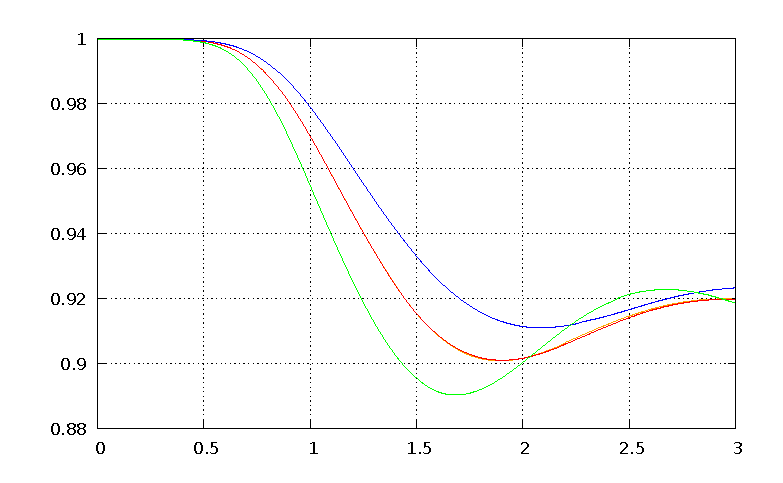
\includegraphics[width=.45\textwidth]
{figures/navier_stokes/2d_rising_bubble_sphericity.ps}
\caption[Navier--Stokes 2d rising bubble sphericity]
{A plot of the sphericity $\strikes$ over time for the simulation in
Figure~\ref{fig:rising_bubble_2d_pressure} for the explicit (orange), implicit
(red), ALE (blue) and antisymmetric (green) schemes.}
\label{fig:rising_bubble_2d_bulk_sphericity}
\end{figure}

\begin{figure}[htbp]
\centering
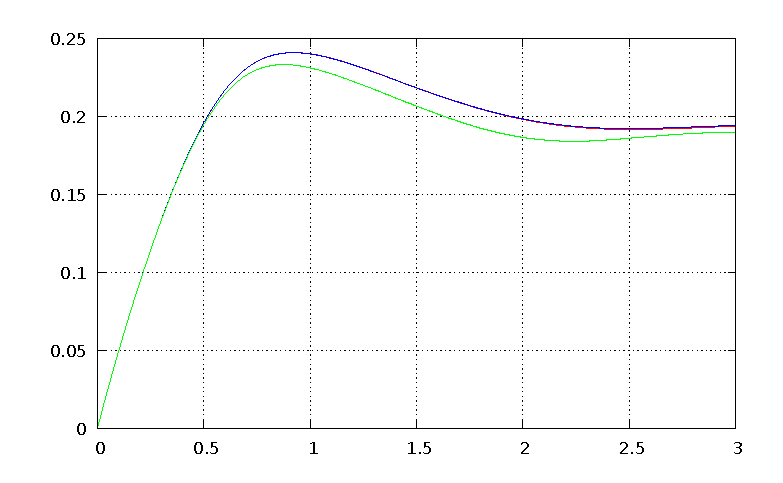
\includegraphics[width=.45\textwidth]
{figures/navier_stokes/2d_rising_bubble_rising_velocity.ps}
\caption[Navier--Stokes 2d rising bubble rising velocity]
{A plot of the rising velocity $V_c$ over time for the simulation in
Figure~\ref{fig:rising_bubble_2d_pressure} for the explicit (orange), implicit
(red), ALE (blue) and antisymmetric (green) schemes.}
\label{fig:rising_bubble_2d_bulk_rising_velocity}
\end{figure}

\begin{figure}[htbp]
\centering
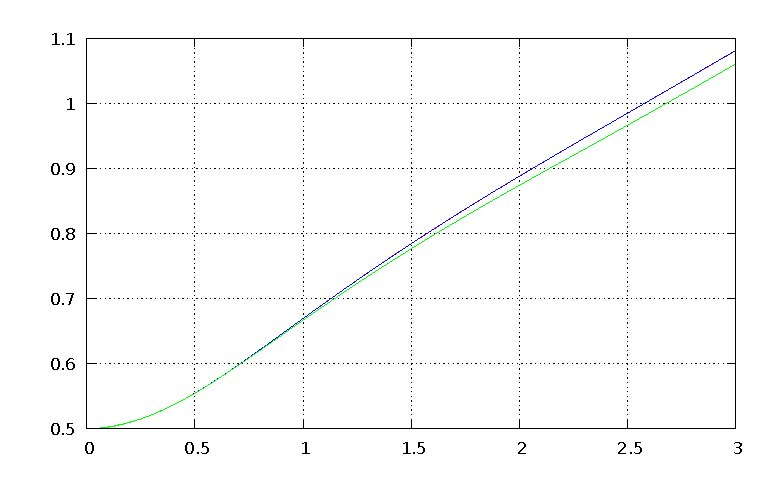
\includegraphics[width=.45\textwidth]
{figures/navier_stokes/2d_rising_bubble_barycenter.ps}
\caption[Navier--Stokes 2d rising bubble barycenter]
{A plot of the barycenter $z_c$ over time for the simulation in
Figure~\ref{fig:rising_bubble_2d_pressure} for the explicit (orange), implicit
(red), ALE (blue) and antisymmetric (green) schemes.}
\label{fig:rising_bubble_2d_bulk_barycenter}
\end{figure}

\begin{figure}[htbp]
\centering
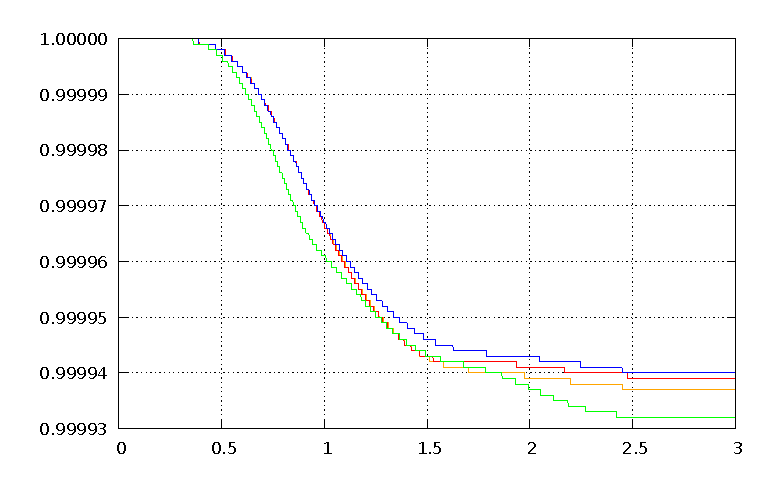
\includegraphics[width=.45\textwidth]
{figures/navier_stokes/2d_rising_bubble_inner_volume.ps}
\caption[Navier--Stokes 2d rising bubble inner area]
{A plot of the relative inner area
$\frac{\mathcal{L}^2(\Omega^m_-)}{\mathcal{L}^2(\Omega^0_-)}$ over time for the
simulation in Figure~\ref{fig:rising_bubble_2d_pressure} for the explicit
(orange), implicit (red), ALE (blue) and antisymmetric (green) schemes.}
\label{fig:rising_bubble_2d_bulk_inner_volume}
\end{figure}